%%%%%%%%%%%%%%%%%%%%%%%%%%%%%%%%%%%%%%%%%%%%%%%%%%%%%%%%%%%%%%%%%%%%%%%%%%%%%%%%
% Template for USENIX papers.
%
% History:
%
% - TEMPLATE for Usenix papers, specifically to meet requirements of
%   USENIX '05. originally a template for producing IEEE-format
%   articles using LaTeX. written by Matthew Ward, CS Department,
%   Worcester Polytechnic Institute. adapted by David Beazley for his
%   excellent SWIG paper in Proceedings, Tcl 96. turned into a
%   smartass generic template by De Clarke, with thanks to both the
%   above pioneers. Use at your own risk. Complaints to /dev/null.
%   Make it two column with no page numbering, default is 10 point.
%
% - Munged by Fred Douglis <douglis@research.att.com> 10/97 to
%   separate the .sty file from the LaTeX source template, so that
%   people can more easily include the .sty file into an existing
%   document. Also changed to more closely follow the style guidelines
%   as represented by the Word sample file.
%
% - Note that since 2010, USENIX does not require endnotes. If you
%   want foot of page notes, don't include the endnotes package in the
%   usepackage command, below.
% - This version uses the latex2e styles, not the very ancient 2.09
%   stuff.
%
% - Updated July 2018: Text block size changed from 6.5" to 7"
%
% - Updated Dec 2018 for ATC'19:
%
%   * Revised text to pass HotCRP's auto-formatting check, with
%     hotcrp.settings.submission_form.body_font_size=10pt, and
%     hotcrp.settings.submission_form.line_height=12pt
%
%   * Switched from \endnote-s to \footnote-s to match Usenix's policy.
%
%   * \section* => \begin{abstract} ... \end{abstract}
%
%   * Make template self-contained in terms of bibtex entires, to allow
%     this file to be compiled. (And changing refs style to 'plain'.)
%
%   * Make template self-contained in terms of figures, to
%     allow this file to be compiled. 
%
%   * Added packages for hyperref, embedding fonts, and improving
%     appearance.
%   
%   * Removed outdated text.
%
%%%%%%%%%%%%%%%%%%%%%%%%%%%%%%%%%%%%%%%%%%%%%%%%%%%%%%%%%%%%%%%%%%%%%%%%%%%%%%%%

\documentclass[letterpaper,twocolumn,10pt]{article}
\usepackage{usenix2019_v3}

% to be able to draw some self-contained figs
\usepackage{tikz}
\usetikzlibrary{quotes}
\usetikzlibrary{calc}
\usetikzlibrary{shapes}
\usetikzlibrary{positioning}
\tikzset{shape example/.style = {
    color=black!50, draw, fill=blue!10,
    inner xsep=1.5cm, inner ysep=0.5cm,
}}
\newcommand{\minus}{\raisebox{0.96pt}{-}}
\usepackage{amsmath}

% inlined bib file
\usepackage{filecontents}

% support CN
\usepackage{CJKutf8}

%-------------------------------------------------------------------------------
\begin{filecontents}{\jobname.bib}
%-------------------------------------------------------------------------------
@Book{arpachiDusseau18:osbook,
  author =       {Arpaci-Dusseau, Remzi H. and Arpaci-Dusseau Andrea C.},
  title =        {Operating Systems: Three Easy Pieces},
  publisher =    {Arpaci-Dusseau Books, LLC},
  year =         2015,
  edition =      {1.00},
  note =         {\url{http://pages.cs.wisc.edu/~remzi/OSTEP/}}
}
@InProceedings{waldspurger02,
  author =       {Waldspurger, Carl A.},
  title =        {Memory resource management in {VMware ESX} server},
  booktitle =    {USENIX Symposium on Operating System Design and
                  Implementation (OSDI)},
  year =         2002,
  pages =        {181--194},
  note =         {\url{https://www.usenix.org/legacy/event/osdi02/tech/waldspurger/waldspurger.pdf}}}
@inbook{10.1145/3335772.3335934,
  author = {Lamport, Leslie},
  title = {Time, clocks, and the ordering of events in a distributed system},
  year = {2019},
  isbn = {9781450372701},
  publisher = {Association for Computing Machinery},
  address = {New York, NY, USA},
  url = {https://doi.org/10.1145/3335772.3335934},
  booktitle = {Concurrency: The Works of Leslie Lamport},
  pages = {179–196},
  numpages = {18}}
\end{filecontents}

%-------------------------------------------------------------------------------
\begin{document}
% \begin{CJK}{UTF8}{gbsn}
%-------------------------------------------------------------------------------

%don't want date printed
\date{}

% make title bold and 14 pt font (Latex default is non-bold, 16 pt)
\title{\Large \bf 寻找一种易理解的共识算法\\
  (扩展版本)}

%for single author (just remove % characters)
\author{
  {\rm Diego Ongaro and John Ousterhout}\\
  Stanford University
  \and
  {\rm Translated into Simplified Chinese from raft.github.io/raft.pdf}\\
  {\rm by xdsdmg@163.com}
} % end author

\maketitle

%-------------------------------------------------------------------------------
\begin{abstract}
  %-------------------------------------------------------------------------------
  Raft是一种管理复制日志的共识算法,它提供了和(multi-)Paxos等效的结果,且它和Paxos一样有效,但结构不同于Paxos,这使得Raft更易理解,且能够为构建实际系统提供更好的基础。为了提高可理解性,Raft将共识划分为Leader选举、日志复制及安全性等核心模块,并且它加强了一致性以减少需要考虑的状态。用户研究表明,对于学生而言,Raft相交于Paxos更易理解。Raft还提供了一种用于改变集群成员的新机制,其使用重叠大多数(overlapping majorities)\footnote{这里翻译得不准确,需要调整}来保证安全性。
\end{abstract}

%-------------------------------------------------------------------------------
\section{Raft共识算法}
%-------------------------------------------------------------------------------

你好呀
A paragraph of text goes here. Lots of text. Plenty of interesting
text. Text text text text text text text text text text text text text
text text text text text text text text text text text text text text
text text text text text text text text text text text text text text
text text text text text text text.
More fascinating text. Features galore, plethora of promises.

\subsection{Raft 基础}
一个Raft集群含有若干个服务节点,通常为$5$个,系统能够容忍最多两个节点发生故障。在任何给定的时间,服务节点的状态为leader、follower及candidate的其中一个。正常运作时,只有一个leader节点,其他节点皆处于follower状态。

Raft将时间分割为任意长度的term,详见图 \ref{fig:term}。term使用连续数字编号。每个term以选举开始,在选举中,一个或多个candidate节点尝试成为leader节点,详见章节 \ref{sec:leader-election}。如果某个candidate节点赢得了选举,那么它将在此term的剩余时间内担任leader节点。在一些情况下,选举会导致投票分裂,term将以没有leader节点的状态结束,然后一个新term(新选举)将快速开始。Raft保证在一个term中至多只有一个leader节点。

不同的服务节点可能在不同的时刻观察到term的变化。term在Raft中作为逻辑时钟\cite{10.1145/3335772.3335934},且服务节点能够根据term检测过期信息,比如过期的leader节点。每个服务节点存储当前的term编号,term编号随时间单调递增。服务节点在相互通信时交换彼此当前的term信息,如果一个服务节点的term小于其他节点的,它会将自己的term更新为较大的值。如果candidate或leader节点发现自己的term已过期,它将立即恢复至follower状态。如果服务节点收到携带过期term的请求,它将拒绝此请求。

\begin{figure}
  \begin{center}
    \resizebox{\linewidth}{!}{
      \begin{tikzpicture}[
          state/.style = {ellipse, draw, minimum width=2cm, minimum height=1cm, align=center, fill=green!20, line width=1pt},
          arrow/.style = {thick,->,>=stealth},
          font = \sffamily
        ]

        % Nodes
        \node[state] (follower) {Follower};
        \node[state, right=of follower, xshift=2cm] (candidate) {Candidate};
        \node[state, right=of candidate, xshift=2cm] (leader) {Leader};

        % Paths between nodes
        \draw[arrow] (follower) -- node[above, align=center] {时间结束,\\开始选举} (candidate);
        \draw[arrow] (candidate) -- node[above, align=center] {收到大多数\\服务节点的投票} (leader);
        \draw[arrow] (candidate) to[bend left] node[below, align=center] {发现当前leader节点\\或更新的term} (follower);
        \draw[arrow] (candidate) edge[loop above] node[align=center] {时间结束,\\新一轮选举} (candidate);
        \draw[arrow] (leader) to[bend right=40] node[above, align=center] {发现具有更高\\term编号的服务节点} (follower);

        % Startup arrow
        \draw[arrow] ($(follower.west)+(-1,1)$) to[bend right=30] (follower.west);
        \node[above, align=center] at ($(follower.west)+(-1,1)$) {开始};

      \end{tikzpicture}
    }
  \end{center}
  \caption{\label{fig:state_tran} 服务节点状态。follower只应答来自其他服务节点的请求。如果一个follower未收到任何通信,它将成为candidate并开始选举。收到来自整个集群大多数服务节点投票的candidate将成为新的leader节点。leader节点通常会一直运作至失败为止。}
\end{figure}

\begin{figure}
  \begin{center}
    \resizebox{\linewidth}{!}{
      \begin{tikzpicture}[node distance=0.5cm, every node/.style={inner sep=0,outer sep=0}][\sffamily]
        % Colors
        \definecolor{blue}{RGB}{0,112,192}
        \definecolor{green}{RGB}{146,208,80}
        \definecolor{myred}{RGB}{255,0,0}

        \fill[blue] (0,0.2) rectangle (0.5,1.2);
        \fill[green] (0.5,0.2) rectangle (1.5,1.2);
        \node[above, font=\itshape] at (0.75, 1.4) {term 1};

        \fill[blue] (1.7,0.2) rectangle (2.1,1.2);
        \fill[green] (2.1,0.2) rectangle (3.9,1.2);
        \node[above, font=\itshape] at (2.8, 1.4) {term 2};

        \fill[blue] (4.1,0.2) rectangle (4.6,1.2);
        \node[above, font=\itshape] at (4.35, 1.4) {t3};

        \fill[blue] (4.8,0.2) rectangle (5.3,1.2);
        \fill[green] (5.3,0.2) rectangle (7,1.2);
        \node[above, font=\itshape] at (5.9, 1.4) {term 4};

        \node[text width=2cm, align=center, anchor=north, font=\small] (elec_1) at (0.25, -0.6) {选举};
        \draw[thick, <-] (0.25,0.2) -- (elec_1.north);

        \node[text width=2cm, align=center, anchor=north, font=\small] (nor_op) at (1.5, -0.6) {正常运行};
        \draw[thick, <-] (1,0.2) -- (nor_op.north);

        \node[align=center, anchor=north, font=\small] (no_em_leader) at (4.35, -0.6) {没有出现\\新的leader节点};
        \draw[thick, <-] (4.35,0.2) -- (no_em_leader.north);

        % Time arrow
        \draw[thick, ->] (-0.5,0) -- (7.5,0) node[right] {terms};
      \end{tikzpicture}
    }
  \end{center}
  \caption{\label{fig:term} 时间被分割为term,并且每个term以选举开始。选举成功后,一个leader节点将管理集群直至term结束,选举也可能失败,在此情况下,term将以没有选举出leader节点结束。不同的节点可能在不同的时刻观察到term的变化。}
\end{figure}

\subsection{Leader选举}
\label{sec:leader-election}

%-------------------------------------------------------------------------------
\section{Footnotes, Verbatim, and Citations}
%-------------------------------------------------------------------------------

Footnotes should be places after punctuation characters, without any
spaces between said characters and footnotes, like so.%
\footnote{Remember that USENIX format stopped using endnotes and is
  now using regular footnotes.} And some embedded literal code may
look as follows.

\begin{verbatim}
int main(int argc, char *argv[]) 
{
    return 0;
}
\end{verbatim}

Now we're going to cite somebody. Watch for the cite tag. Here it
comes. Arpachi-Dusseau and Arpachi-Dusseau co-authored an excellent OS
book, which is also really funny~\cite{arpachiDusseau18:osbook}, and
Waldspurger got into the SIGOPS hall-of-fame due to his seminal paper
about resource management in the ESX hypervisor~\cite{waldspurger02}.

The tilde character (\~{}) in the tex source means a non-breaking
space. This way, your reference will always be attached to the word
that preceded it, instead of going to the next line.

And the 'cite' package sorts your citations by their numerical order
of the corresponding references at the end of the paper, ridding you
from the need to notice that, e.g, ``Waldspurger'' appears after
``Arpachi-Dusseau'' when sorting references
alphabetically~\cite{waldspurger02,arpachiDusseau18:osbook}.

It'd be nice and thoughtful of you to include a suitable link in each
and every bibtex entry that you use in your submission, to allow
reviewers (and other readers) to easily get to the cited work, as is
done in all entries found in the References section of this document.

Now we're going take a look at Section~\ref{sec:figs}, but not before
observing that refs to sections and citations and such are colored and
clickable in the PDF because of the packages we've included.

%-------------------------------------------------------------------------------
\section{Floating Figures and Lists}
\label{sec:figs}
%-------------------------------------------------------------------------------


%---------------------------
\begin{figure}
  \begin{center}
    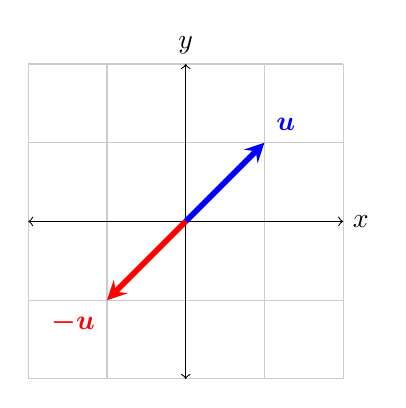
\begin{tikzpicture}
      \draw[thin,gray!40] (-2,-2) grid (2,2);
      \draw[<->] (-2,0)--(2,0) node[right]{$x$};
      \draw[<->] (0,-2)--(0,2) node[above]{$y$};
      \draw[line width=2pt,blue,-stealth](0,0)--(1,1)
      node[anchor=south west]{$\boldsymbol{u}$};
      \draw[line width=2pt,red,-stealth](0,0)--(-1,-1)
      node[anchor=north east]{$\boldsymbol{-u}$};
    \end{tikzpicture}
  \end{center}
  \caption{\label{fig:vectors} Text size inside figure should be as big as
    caption's text. Text size inside figure should be as big as
    caption's text. Text size inside figure should be as big as
    caption's text. Text size inside figure should be as big as
    caption's text. Text size inside figure should be as big as
    caption's text. }
\end{figure}




%% %---------------------------


Here's a typical reference to a floating figure:
Figure~\ref{fig:vectors}. Floats should usually be placed where latex
wants then. Figure\ref{fig:vectors} is centered, and has a caption
that instructs you to make sure that the size of the text within the
figures that you use is as big as (or bigger than) the size of the
text in the caption of the figures. Please do. Really.

In our case, we've explicitly drawn the figure inlined in latex, to
allow this tex file to cleanly compile. But usually, your figures will
reside in some file.pdf, and you'd include them in your document
with, say, \textbackslash{}includegraphics.

Lists are sometimes quite handy. If you want to itemize things, feel
free:

\begin{description}

  \item[fread] a function that reads from a \texttt{stream} into the
        array \texttt{ptr} at most \texttt{nobj} objects of size
        \texttt{size}, returning returns the number of objects read.

  \item[Fred] a person's name, e.g., there once was a dude named Fred
        who separated usenix.sty from this file to allow for easy
        inclusion.
\end{description}

\noindent
The noindent at the start of this paragraph in its tex version makes
it clear that it's a continuation of the preceding paragraph, as
opposed to a new paragraph in its own right.


\subsection{LaTeX-ing Your TeX File}
%-----------------------------------

People often use \texttt{pdflatex} these days for creating pdf-s from
tex files via the shell. And \texttt{bibtex}, of course. Works for us.

%-------------------------------------------------------------------------------
\section*{Acknowledgments}
%-------------------------------------------------------------------------------

The USENIX latex style is old and very tired, which is why
there's no \textbackslash{}acks command for you to use when
acknowledging. Sorry.

%-------------------------------------------------------------------------------
\section*{Availability}
%-------------------------------------------------------------------------------

USENIX program committees give extra points to submissions that are
backed by artifacts that are publicly available. If you made your code
or data available, it's worth mentioning this fact in a dedicated
section.

%-------------------------------------------------------------------------------
\bibliographystyle{plain}
\bibliography{\jobname}

%%%%%%%%%%%%%%%%%%%%%%%%%%%%%%%%%%%%%%%%%%%%%%%%%%%%%%%%%%%%%%%%%%%%%%%%%%%%%%%%
% \end{CJK}
\end{document}
%%%%%%%%%%%%%%%%%%%%%%%%%%%%%%%%%%%%%%%%%%%%%%%%%%%%%%%%%%%%%%%%%%%%%%%%%%%%%%%%

%%  LocalWords:  endnotes includegraphics fread ptr nobj noindent
%%  LocalWords:  pdflatex acks
